%\vspace{-1em}
\subsection{FPGA Implementation Details} \label{sec:fpga}
%\vspace{-0.5em}

Field-Programmable Gate Arrays (FPGA) are an alternative to commonly used Graphics Processing Units (GPU) for accelerated processing of compute intensive machine learning workloads. The custom logic fabric of an FPGA enables the design of specialized compute units, which is very advantageous when working on extremely low-precision and irregular numeric formats, such as 2 bit numbers. Thanks to the microarchitectural flexibility advantage, it is possible to achieve near linear speed-up when lowering the precision of data that is read from the memory. This has been shown recently for stochastic gradient descent (SGD) when training linear models~\cite{zhang2017zipml, kara2017fpga}. In this work, we use the open-source FPGA implementation from the mentioned works and modify it to perform IHT.

In terms of the computation, we need to modify two parts of the design to convert it from performing SGD to IHT: 1) Instead of updating the model after a mini-batch count is reached, we update it after all samples are processed and the true gradient is available. 2) After each epoch, we perform a binary search on the updated model to find the threshold value satisfying that only top $S$ values are larger than the  threshold.

\begin{figure}[t!]
\centering
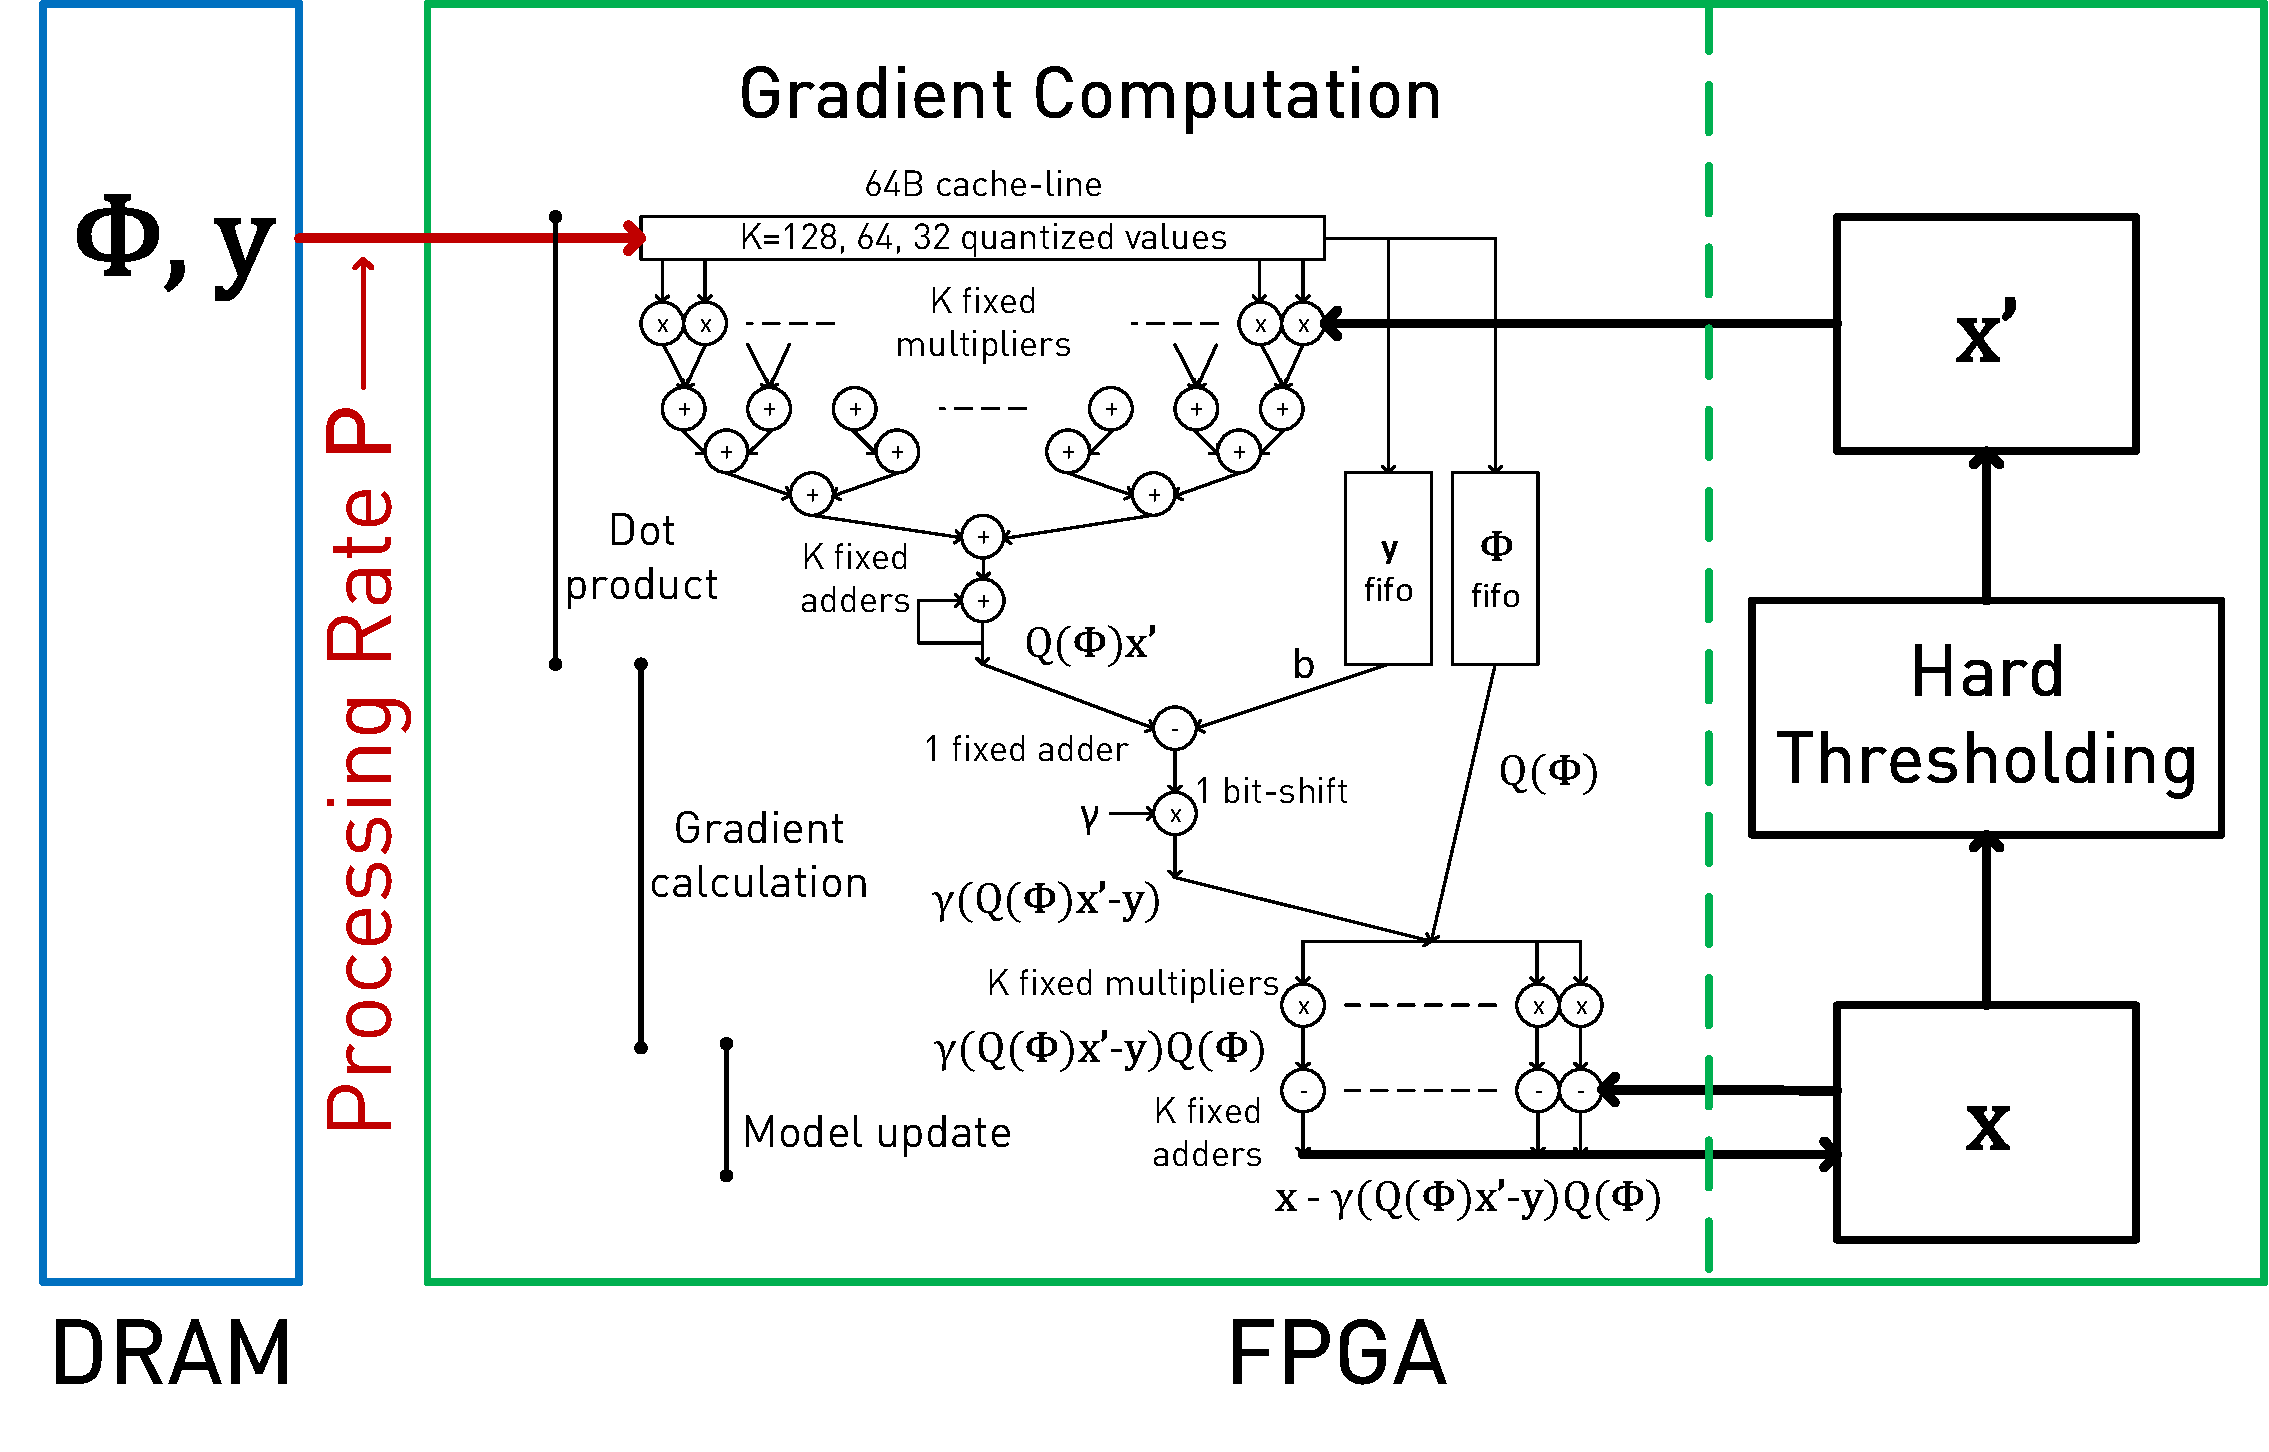
\includegraphics[width=0.5\textwidth, angle=0]{../figs/niht_fpga.pdf}
\caption{IHT on an FPGA-based system.}
\label{fig:fpga}
\end{figure}


{\bf Performance analysis} The gradient computation unit as shown in Fig.~\ref{fig:fpga} reads the measurement matrix ${\bf \Phi}$ and the measurements ${\bf y}$ from main memory and keeps ${\bf x}$ in on-chip memory. 
We note that transferring ${\bf \Phi}$ from main memory will be necessary in most practical settings, where the matrix ${\bf \Phi}$ is too large to fit onto the FPGA. 
The FPGA is able to process data from memory at a rate of ${\bf P}=12.8\,GB/s$. 
Thus, performance will be bound on this rate ${\bf P}$ for processing ${\bf \Phi}$ and ${\bf y}$, which becomes the system bottleneck. The time for each iteration is given by 
$T = size({\bf \Phi})/{\bf P}$, since $size({\bf y}) \ll size({\bf \Phi})$. 
We can achieve significant speed-up by quantizing ${\bf \Phi}$, simply because we reduce the amount of data to be transferred: more entries arrive with each transfer from main memory. 
%, because the time for each epoch is given by
%$T = size({\bf \Phi})/{\bf P}$, since $size({\bf y}) \ll size({\bf \Phi})$. The essential idea behind achieving %linear speed-up is keeping ${\bf P}$ constant as the precision of ${\bf \Phi}$ is lowered (${\bf P}\to \land \, %size({\bf \Phi})\downarrow$), which leads to more values arriving within each transfer from main memory. 
The processing rate ${\bf P}$ can be kept constant on an FPGA, because we can adapt the gradient computation unit's microarchitecture and increase its internal parallelism to handle more values per incoming line. 

{\bf Computing ${\bf \Phi}$ on the fly} The above analysis focuses on the case when ${\bf \Phi}$ 
is stored in main memory, in which case quantization helps to reduce the amount of 
data transferred between the main memory and FPGA. In some applications, ${\bf \Phi}$
can be calculated on the fly, inside the FPGA. Also in this case, quantization can help 
achieve better performance.
The reason why quantizing ${\bf \Phi}$ helps, even if it can be calculated on the fly, is
that a quantized ${\bf \Phi}$ saves many crucial resources (e.g., multipliers) that
are limited on an FPGA. These resource savings are very important in achieving a higher 
internal parallelism, for instance, to speed up the computation of ${\bf \Phi}\times{\bf x}$. 
For example, it has been shown by~\cite{kara2017fpga} that to go from a 64-value dot product to 128-value
dot product on an FPGA, it is necessary to lower the precision of one side of the dot product to 2-bits.
